\def\year{2018}\relax
%File: formatting-instruction.tex
\documentclass[letterpaper]{article} %DO NOT CHANGE THIS
\usepackage{aaai18}  %Required
\usepackage{times}  %Required
\usepackage{helvet}  %Required
\usepackage{courier}  %Required
\usepackage{url}  %Required
\usepackage{graphicx}  %Required
%Non aaai-required
\usepackage{booktabs}
\usepackage{cleveref}
\usepackage{xcolor} 
\usepackage{eso-pic}
\usepackage{xspace}
\usepackage{float}
\usepackage{tcolorbox}
\usepackage{epsfig}
\usepackage{amsmath}
\usepackage{amssymb}
\usepackage{color}
\usepackage{tabu}
\usepackage{multirow}
\usepackage{pifont}% http://ctan.org/pkg/pifont
\usepackage{tikz}
\usepackage{pgfplots}
\usepackage{tikz}
\frenchspacing  %Required
\setlength{\pdfpagewidth}{8.5in}  %Required
\setlength{\pdfpageheight}{11in}  %Required
%PDF Info Is Required:
  \pdfinfo{
/Title (Speech-Based Visual Question Answering)
/Author (Anonymous Authors)}
\setcounter{secnumdepth}{0}
\usepgfplotslibrary{external}
\usetikzlibrary{positioning}
\graphicspath{{./images/}}
\pgfplotsset{compat=1.13}

\newcommand*{\ityping}{
\includegraphics[scale=0.02]{7.png}}
\newcommand*{\ispeaking}{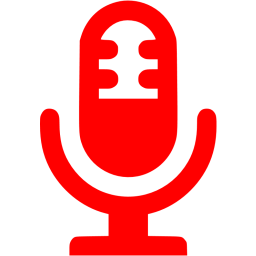
\includegraphics[scale=0.03]{6.png}}
\newcommand{\YES}{\ding{51}}
\newcommand{\NO}{\ding{55}}
\newcommand{\todo}[1]{\textcolor{blue}{#1}}
\newcommand{\vect}[1]{\mathbf{#1}}
\DeclareMathOperator*{\Unif}{U}
\newcommand{\dengxincomment}[1]{\textcolor{blue}{\textit{#1}}}
\newcommand{\tedcomment}[1]{\textcolor{green}{\textit{#1}}}
\newcommand{\ttcomment}[1]{\textcolor{purple}{\textit{#1}}}

\begin{document}
\title{Speech-Based Visual Question Answering}
%%% Commented out for Arxiv submission
%\titlenote{Produces the permission block, and
%  copyright information}
%\subtitlenote{The full version of the author's guide is available as
%  \texttt{acmart.pdf} document}

% \author{Ted Zhang\\
% KU Leuven\\
% tedz.cs@gmail.com}

% \author{Dengxin Dai}
% \affiliation{%
%   \institution{ETH Zurich}
% }
% \email{dai@vision.ee.ethz.ch}

% \author{Tinne Tuytelaars}
% \affiliation{%
%   \institution{KU Leuven}
% }
% \email{tinne.tuytelaars@esat.kuleuven.be }

% \author{Marie-Francine Moens}
% \affiliation{%
%   \institution{KU Leuven}
% }
% \email{sien.moens@cs.kuleuven.be}

% \author{Luc Van Gool}
% \affiliation{%
%   \institution{ETH Zurich}
% }
% \email{vangool@vision.ee.ethz.ch}
\maketitle
\begin{abstract}
This paper introduces speech-based visual question answering (VQA), the task of generating an answer given an image and a spoken question. Our work is the first study of speech-based VQA with the intention of providing insights for applications such as speech-based virtual assistants. Two methods are studied: an end to end, deep neural network that directly uses audio waveforms as input versus a pipelined approach that performs ASR (Automatic Speech Recognition) on the question, followed by text-based visual question answering. Our main findings are 1) speech-based VQA achieves slightly worse results than the extensively-studied VQA with noise-free text and 2) the end-to-end model is competitive even though it has a simple architecture. Furthermore, we investigate the robustness of both methods by injecting various levels of noise into the spoken question and find speech-based VQA to be tolerant of noise at reasonable levels. The speech dataset, code, and supplementary material will be released to the public.\footnote{http://data.vision.ee.ethz.ch/daid/VQA/SpeechVQA.zip}

\end{abstract}
\label{sec:intro}
\section{Introduction}

The recent years have witnessed great advances in computer vision, natural language processing, and speech recognition thanks to the advances in deep learning \cite{lecun2015deep} and abundance of data \cite{imagenet:2015}, \cite{VQA}. This is evidenced not only by the surge of academic papers, but also by the world-wide industry interests. The convincing successes in these individual fields naturally raise the potentials of further integration towards solutions to more general AI problems. Much work has been done to integrate vision and language, resulting in a wide collection of successful applications such as image/video captioning \cite{show:tell:caption}, movie-to-book alignment \cite{align:bookmovie}, and visual question answering (VQA) \cite{VQA}. However, the importance of integrating vision and speech has remained relatively unexplored.

Pertaining to practical applications, voice-user interface (VUI) has become more commonplace, and people are increasingly taking advantage of its characteristics; it is natural, hands-free, eyes-free, far more mobile and even faster than typing on certain devices \cite{speech:faster}. As many of our daily tasks are relevant to visual scenes, there is a strong need to have a VUI to talk to pictures or videos directly, be it for communication, cooperation, or guidance. Speech-based VQA can be used to assist blind people in performing ordinary tasks, and to dictate robotics in real visual scenes in a hand-free manner such as clinical robotic surgery.


%Diagram
\begin{figure}[t]
\centering
\begin{tikzpicture}[
bluesquare/.style={rectangle, draw=blue!70, fill=blue!4, very thick, minimum size=5mm},
greensquare/.style={rectangle, draw=green!70, fill=green!4, very thick, minimum size=5mm},
magsquare/.style={rectangle, draw=magenta!70, fill=magenta!4, very thick, minimum size=5mm},
empty/.style={rectangle, very thick, minimum size=7mm},
]

%Nodes TextMod
\node[magsquare, outer sep=5pt]      (model2)           {TextMod};
\node[empty] (answer2) [right=of model2] {pizza};
\node[inner sep=5pt] (pizza2)  [above=of model2] {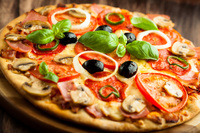
\includegraphics[width=.1\textwidth]{pizzas.jpg}};
\node[greensquare, outer sep=5pt, label=below:what food is this?]    (asr)  [left=1cm of model2] {ASR}; 
\node[inner sep=5pt] (wav2)  [above=of asr] {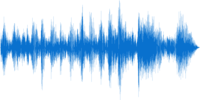
\includegraphics[width=.1\textwidth]{wavs.png}}; 

%Nodes SpeechMod
\node[inner sep=5pt] (pizza1)  [below=of model2] {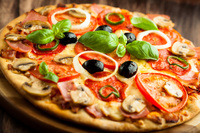
\includegraphics[width=.1\textwidth]{pizzas.jpg}};
\node[bluesquare, outer sep=5pt]   [below=of pizza1]   (model1)                      {SpeechMod};
\node[empty] (answer1) [right=of model1] {pizza};
\node[inner sep=5pt] (wav1)  [left=of model1] {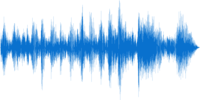
\includegraphics[width=.1\textwidth]{wavs.png}};


% %Lines
\draw[->] (wav1.east) -- (model1.west);
\draw[->] (pizza1.south) -- (model1.north);
\draw[->] (model1.east) -- (answer1.west);

\draw[->] (wav2.south) -- (asr.north);
\draw[->] (asr.east) -- (model2.west);
\draw[->] (pizza2.south) -- (model2.north);
\draw[->] (model2.east) -- (answer2.west);

\end{tikzpicture}
\caption{An example of speech-based visual question answering and the two method in this study. A spoken question \emph{what food is this?} is asked about the picture, and the system is expected to generate the answer \emph{pizza}. TextMod uses a pipelined approach with ASR to retrieve the text first, while SpeechMod utilizes audio inputs directly.}
\label{fig:models}
\end{figure}

This work investigates the potential of integrating vision and speech in the context of VQA. A spoken version of the \textit{VQA1.0} dataset is generated to study two different methods of speech-based question answering. One method is an end-to-end approach based on a deep neural network architecture, and the other uses an ASR to first transcribe the text from the spoken question, as shown in \Cref{fig:models}. The former approach is particularly useful for languages that are not serviced by popular ASR systems, i.e. minor languages that have scarce text-speech aligned training data.

The \textbf{main contributions} of this paper are three-fold: \textbf{1)} We introduce an end-to-end model that directly produces answers from auditory input, without transformations into intermediate pre-learned representations, and compare this with a pipelined approach that first converts speech to text. \textbf{2)} We inspect the performance impact of having different levels of background noise mixed with the original utterances. \textbf{3)} We release the speech dataset, roughly 200 hours of synthetic audio data and 1 hour of real speech data, to the public.

To be certain, readers will notice that our models are simple. The emphasis of this paper is not on achieving the best performance for either the end-to-end nor the pipelined approach. Rather, it is to provide a baseline, to induct speech-based visual question answering into the multimedia research domain, and to provide some insights in this topic.

The paper is structured as follows: \Cref{sec:related} introduces the related work. \Cref{sec:method} is devoted to our methods, which is followed by Section \Cref{sec:data} for our data. \Cref{sec:experiment} then presents our experimental settings, followed by \Cref{sec:discussion} for discussions. Finally, \Cref{sec:conclusion} concludes the paper.   

\section{Related Works}
\label{sec:related}
Our work is generally relevant to visual question answering, the integration of vision and speech, and end-to-end speech recognition.

\subsection{Visual Question Answering}
The initial introduction of VQA into the AI community \cite{realtime:vqa}, \cite{daquar} was motivated by a desire to build intelligent systems that can understand the world more holistically. In order to complete the task of VQA, it was both necessary to understand a textual question and a visual scene. However, it was not until the introduction of \textit{VQA 1.0} \cite{VQA} that the application took mainstream in the computer vision and natural language processing (NLP) communities.

Recently, popular topics of exploration have been on the development of attention models. Attention models were popularized by its success with the NLP community in machine translation \cite{nmt:joint:align}. They eventually found a place in the computer vision community in works such as \cite{recurrent:visual:attn}, \cite{dnn:selective:attn}, and \cite{show:attend:tell}. Within the context of visual question answering, attention mechanisms `show' a model where to look when answering a question. Stacked Attention Network \cite{vqa:stackedattn} learns an attention mechanism based on the of the question's encoding to determine the salient regions in an image. More sophisticated attention-centric models such as \cite{vqa:dualattn,vqa:hieco} and \cite{vqa:dynamicmemory} were since then developed.

Other points of research are based on the pooling mechanism that combines the language component with the vision components. Many models \cite{vqa:spatial:attn} \cite{vqa:simp} \cite{vqa:stackedattn} use an element-wise multiplication to pool these modalities, \cite{vqa:hieco} and Fukui et al. \cite{multimodal:pooling} have shown much success in using more complex methods. Our work differs from theirs in that we do not try to improve the performance of the VQA model by adding attention mechanisms or augmenting the pooling techniques.


\subsection{Integration of Speech and Vision}
The works also relevant to ours are those integrating speech and vision. Pixeltone \cite{pixel:tone}
and Image spirit \cite{image:spirit} are examples that use voice
commands to guide image processing and semantic segmentation. There is also academic work \cite{show:tell} \cite{speech:anno:img} \cite{speech:retri:img} and an app \cite{smile} that use speech to provide image descriptions. Their tasks and algorithms are both different from ours. We study the potential of integrating speech and vision in the context of VQA and aim to learn a joint understanding of speech and vision. Those approaches, however, use speech recognition for data collection or result refinement.

Our work also shares similarity with visual-grounded speech understanding or recognition. The closest one in this vein is \cite{speech:caption}, in which a deep model is learned with speeches about image captions for speech-based image retrieval. In a broader context of integration of sound and vision, Soundnet \cite{soundnet} transfers visual information into sound representations, but this differs from our work because their end goal is to label a sound.

\subsection{End-To-End Speech Recognition}
In the past decade, deep learning has allowed many fields in artificial intelligence to replace traditional hand-crafted features and pipeline systems with end-to-end models. Since speech recognition is typically thought of as a sequence to sequence transduction problem, i.e. given an input sequence, predict an output sequence, the application of LSTM and the CTC \cite{rnn:discrimspotting}, \cite{ctc} promptly showed the success needed to justify its superiority over traditional methods. Current state of the art ASR systems such as DeepSpeech2 \cite{deepspeech2} uses stacked Bi-directional Recurrent Neural Networks (RNNs) in conjunction with Convolutional Neural networks (CNNs) because these deep neural architectures all share the property of being able to perform back propagation. While our work does not attempt sequence to sequence prediction nor make use of CTCs, our approach and the integration of speech with vision is nevertheless made possible by the same underlying principle of the works listed above.


%Model Architecture
\begin{figure}[t]
\centering
\begin{tikzpicture}[
inps/.style={rectangle, draw=black!60, very thick, minimum size=10mm},
rect/.style={rectangle, draw=black!60, very thick, minimum size=5mm},
circ/.style={circle, draw=black!60, very thick, minimum size=5mm},
empty/.style={rectangle, very thick, minimum size=5mm},
]

\node[empty]      (central)             {};

%TextMod
%Nodes
\node[circ]      (1main)          [left =15mm of central]      {.};
% Linguistic
\node[rect]      (1ldense)        [above right=3mm of 1main]        {Dense};
\node[rect]      (1lstm)     [above=2mm of 1ldense]           {LSTM};
\node[rect]      (1emb)          [above=2mm of 1lstm]      {Embedding};
\node[empty]      (1linput)    [above=1mm of 1emb]            {Text};
% Visual
\node[rect]      (1vdense)       [above left=3mm of 1main]         {Dense};
\node[empty]        (1vinput)  [above=1mm of 1vdense] {Image};
% Combined
\node[rect, outer sep=2pt]      (1cdense1)        [below=2mm of 1main]        {Dense};
\node[rect, outer sep=2pt]      (1cdense2)        [below=2mm of 1cdense1]        {Dense};
\node[empty] (1answer) [below=2mm of 1cdense2] {output};

% Lines
\draw[->] (1emb.south) -- (1lstm.north);
\draw[->] (1lstm.south) -- (1ldense.north);
\draw[->] (1ldense.south) -- (1main.east);

\draw[->] (1vdense.south) -- (1main.west);

\draw[->] (1main.south) -- (1cdense1.north);
\draw[->] (1cdense1.south) -- (1cdense2.north);
\draw[->] (1cdense2.south) -- (1answer.north);

%SpeechMod
%Nodes
\node[circ]      (2main)          [right =15mm of central]      {.};
% Linguistic
\node[rect]      (2ldense)        [above right=3mm of 2main]        {Dense};
\node[rect]      (2lstm)     [above=2mm of 2ldense]           {LSTM};
\node[rect]      (convs)          [above=2mm of 2lstm, align=center]      {Conv Layers\\(Dimensions\\in \Cref{table:convdims})};
\node[empty]    (2linput)         [above=1mm of convs]      {Audio};
% Visual
\node[rect]      (2vdense)       [above left=3mm of 2main]         {Dense};
\node[empty]     (2vinput)  [above=1mm of 2vdense] {Image};
% Combined
\node[rect, outer sep=2pt]      (2cdense1)        [below=2mm of 2main]        {Dense};
\node[rect, outer sep=2pt]      (2cdense2)        [below=2mm of 2cdense1]        {Dense};
\node[empty] (2answer) [below=2mm of 2cdense2] {output};

\draw[->] (convs.south) -- (2lstm.north);
\draw[->] (2lstm.south) -- (2ldense.north);
\draw[->] (2ldense.south) -- (2main.east);

\draw[->] (2vdense.south) -- (2main.west);

\draw[->] (2main.south) -- (2cdense1.north);
\draw[->] (2cdense1.south) -- (2cdense2.north);
\draw[->] (2cdense2.south) -- (2answer.north);


\end{tikzpicture}
\caption{TextMod (left) and SpeechMod (right) architectures}
\label{fig:modarc}
\end{figure}

\section{Model}
\label{sec:method}
Two models are employed in this work, they will be referred to henceforth as TextMod and SpeechMod. TextMod and SpeechMod only differ in their language components, keeping rest of the architecture the same. On the language side, TextMod takes as input a series of one-hot encodings, followed by an embedding layer that is learned from scratch, a LSTM encoder, and a dense layer. It is similar to \cite{VQA} with some minor adjustments.

The language side of SpeechMod takes as input the raw waveform, and pushes it through a series of 1D convolutions. After the CNN layers follows a LSTM. The LSTM serves the same purpose as in TextMod, which is to interpret and encode the sequence meaningfully into a single vector.

A CNN is used here because of its ability to reduce the dimensionality of data while finding salient patterns. One could directly feed the input waveform to a LSTM, but a LSTM will be unable to learn from sequences that are excessively long. The maximum length of an input waveform has 107,360 elements, which corresponds to 6.7 seconds of audio, while the minimum length is 10,080, which corresponds to 0.63 seconds of audio. A LSTM (or any recurrent net) would not be able to deal with even the minimum length of data, so dimensionality reduction is a necessity. At each convolution layer, I halve the filter length and double the number of filters. This is done for simplicity rather than for performance optimization. The main consideration taken in choosing the parameters is that the last convolution should output dimensions of (x, 512), where $x$ must be a positive integer. $x$ represents the length of a sequence of 512-dim vectors. The sequence is then fed into an LSTM, which then outputs a single vector of (512). Thus, $x$ should not be too big, and the CNN parameters are chosen to ensure a sensible sequence length. The exact dimensions of the convolution layers are shown in \Cref{table:convdims}. The longest and shortest waveforms (length of 107,360 and 10,080) correspond to final convolution outputs of size (13, 512) and (1, 512) respectively. 512 is used as the dimension of the LSTM to be consistent with TextMod and the original VQA baseline.

On the visual side, both models ingest as input the 4,096 dimensional vector of the last layer of VGG19 \cite{vgg16} followed by a single dense layer. After both visual and linguistic representations are computed, they are merged using element-wise multiplication, a dense layer, and an output layer. The full architecture of both these models are seen in \Cref{fig:modarc}, where $\displaystyle\odot$ is the symbol for element-wise multiplication. After merging the language and visual components of each model, two dense layers are stacked. The last dense layer outputs a probability distribution over the number of output classes, and the answer corresponding to the element with the highest probability is selected.

The architectures presented in this chapter were chosen for two main reasons: simplicity and similarity. First, the intention is to keep the model complexity low - there are no complex multimodal merging strategies, attention mechanisms, residual layers, or pre-trained embeddings. In order to establish a baseline for speech-based VQA, it is necessary to use only the bare minimum components. TextMod, as mentioned before, is similar to the original VQA baseline, which is well referenced and remains the simplest architecture on \textit{VQA1.0}. SpeechMod, despite its many convolution layers, uses minimal components too. Long inputs sequences such as audio waveforms must have their dimensionality reduced. While LSTMs can reduce dimensions, it does so in a single layer, which prevents the step-wise and gradual learning of hierarchical representations. Vanilla networks are unable to deal with variable length inputs, and like with LSTMs, the input dimension of waveforms are too long to handle computationally and difficult to learn from. In contrast, CNNs can gradually reduce dimensions while learning hierarchical features, and cope well with variable length inputs. Second, it is important that TextMod and SpeechMod differ from each other as little as possible. Similarity between models allows one to locate the source of discrepancies and helps produce a more rigorous comparison. The only difference in the two models is replacing an embedding layer with a series of convolution layers. In the architecture implementations, all the other layers have the same dimensions too.


\begin{table*}[!ht]
\centering
\caption{Dimensions for the conv layers. Example shown with a 2 second long audio waveform, sampled at 16 kHz. The final output dimensions are (3, 512)}
\label{table:convdims}
\begin{tabular}{l|c|c|c|c|c|c|c|c|c}
Layer         & \multicolumn{1}{l|}{conv1} & \multicolumn{1}{l|}{pool1} & \multicolumn{1}{l|}{conv2} & \multicolumn{1}{l|}{pool2} & \multicolumn{1}{l|}{conv3} & \multicolumn{1}{l|}{pool3} & \multicolumn{1}{l|}{conv4} & \multicolumn{1}{l|}{pool4} & \multicolumn{1}{l}{conv5} \\ \hline
Input Dim     & 32,000                      & 16,000                      & 4,000                       & 2,000                       & 500                        & 250                        & 62                         & 31                         & 7                         \\
\# Filters    & 32                         & 32                         & 64                         & 64                         & 128                        & 128                        & 256                        & 256                        & 512                       \\
Filter Length & 64                         & 4                          & 32                         & 4                          & 16                         & 4                          & 8                          & 4                          & 4                         \\
Stride        & 2                          & 4                          & 2                          & 4                          & 2                          & 4                          & 2                          & 4                          & 2                         \\
Output Dim    & 16,000                      & 4,000                       & 2,000                       & 500                        & 250                        & 62                         & 31                         & 7                          & 3                        
\end{tabular}
\end{table*}



\section{Data}
\label{sec:data}
We chose to use \textit{VQA 1.0} Open-Ended dataset, for its numerous training examples and familiarity to those working in question answering. To avoid ambiguity, from here onwards \textit{VQA 1.0} refers to the dataset, and VQA refers to the task of visual question answering. The dataset contains 248,349 questions in the training set, 121,512 in validation set, and 60,864 in the test-dev set. The complete test set contains 244,302 questions, but because the evaluation server allows for only one submission, we instead evaluate on test-dev, which has no such limit. Both \textit{train} + \textit{val} are used during the training but questions which do not contain the 1000 most common answers are filtered out. This leaves 320,029 questions for training.

Amazon Polly API is used to generate audio files for each question.~\footnote{The voice of Joanna is used: \url{https://aws.amazon.com/polly/}} The generated speech is in mp3 format, then sampled into waveform format at 16 kHz. 16 kHz was chosen due to its common usage among the speech community, but also because the model used to transcribe speech was trained on 16 kHz audio waveforms. It is worthwhile to note that the audio generator uses a female voice, thus the training and testing data are all with the same voice, except for the examples we’ve recorded, which is covered below. The full Amazon Polly speech dataset will be made available to the public.

The noise we mixed with the original speech files is selected randomly from the Urban8K dataset \cite{urban8k}. This dataset contains 10 categories: air conditioner, car horn, children playing, dog bark, drilling, engine idling, gun shot, jackhammer, siren, and street music. Some clips are soft enough in volume and thus considered background noise, others are loud enough to be considered foreground noise. For each original audio file, a random noise file is selected, and combined to produce a corrupted question file according to the weighting scheme:
\begin{displaymath}
  W_{corrupted} = (1-\mathit{NL})*W_{original}  + \mathit{NL}*W_{noise}
\end{displaymath}
where \textit{NL} is the noise level. The noise audio files are subsampled to 16 kHz in order to match that of the original audio file, and is clipped to also match the spoken question length. When the spoken question is longer than the noise file, the noise file is repeated until its duration exceeds that of the spoken question. Both files are normalized before being combined so that contributions are strictly proportional to the noise level chosen. We choose 5 noise levels to mix together: 10\%-50\%, at 10\% intervals. Anything beyond 50\% is unrealistic. A visualization of different noise levels can be seen in \Cref{fig:specs} and its corresponding audio clips can be found online.\footnote{https://soundcloud.com/sbvqa/sets/speechvqa}

%Diagram
\begin{figure}[t]
\centering
\begin{tikzpicture}[
scale=0.66,
every node/.style={scale=0.66},
squarednode/.style={rectangle, draw=red!70, fill=red!4, very thick, minimum size=5mm},
empty/.style={rectangle, very thick, minimum size=1mm},
]
%Nodes
\node (-center) [empty]      (model)                      {};


\node[inner sep=0.5pt, label=below:what is the number of the bus] (2n0)  [below=8mm of model] {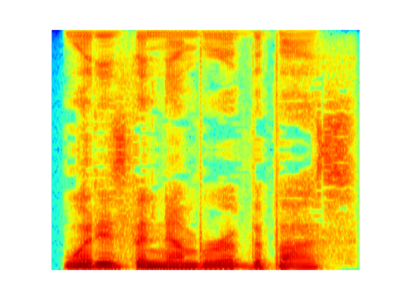
\includegraphics[width=0.2\textwidth]{2_noise0.png}};
\node[inner sep=0.5pt, label=below:what is the number of the boss] (2n30)  [below=8mm of 2n0] {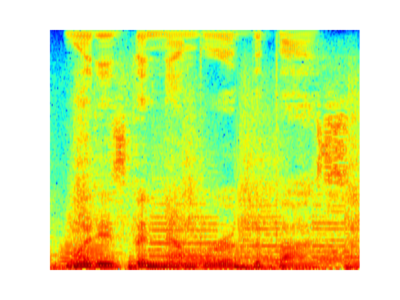
\includegraphics[width=0.2\textwidth]{2_noise30.png}};
\node[inner sep=0.5pt, label=below:where is it] (2n50)  [below=8mm of 2n30] {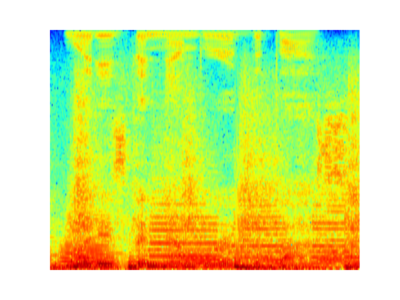
\includegraphics[width=0.2\textwidth]{2_noise50.png}};
\node[inner sep=0.5pt, label=below:what is the number of the boss] (2r)  [below=8mm of 2n50] {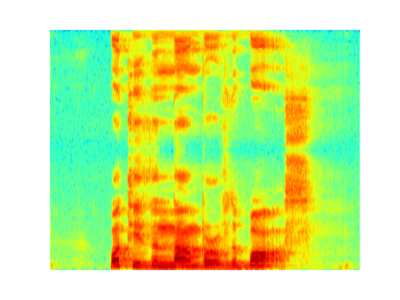
\includegraphics[width=0.2\textwidth]{2_recorded.png}};

\node[inner sep=0.5pt, label=below:what time of day is it] (1n0)  [left=4mm of 2n0] {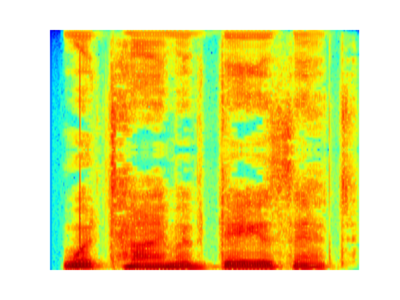
\includegraphics[width=0.2\textwidth]{1_noise0.png}};
\node[inner sep=0.5pt, label=below:what time of day isn't] (1n30)  [left=4mm of 2n30] {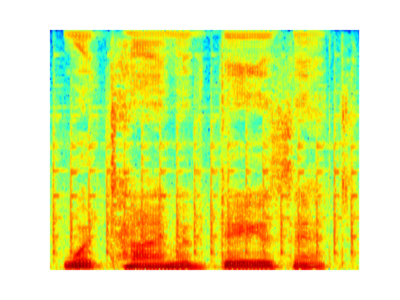
\includegraphics[width=0.2\textwidth]{1_noise30.png}};
\node[inner sep=0.5pt, label=below:what time and day isn't] (1n50)  [left=4mm of 2n50] {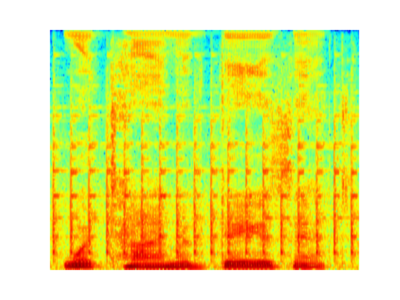
\includegraphics[width=0.2\textwidth]{1_noise50.png}};
\node[inner sep=0.5pt, label=below:what time of day is it] (1r)  [left=4mm of 2r] {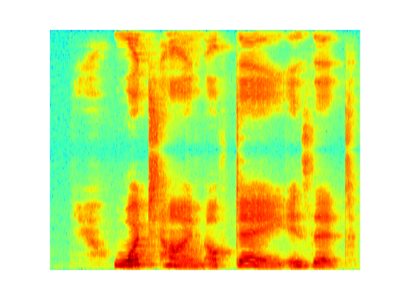
\includegraphics[width=0.2\textwidth]{1_recorded.png}};


\node[inner sep=0.5pt, label=below:are there clouds on the sky] (3n0)  [right=4mm of 2n0] {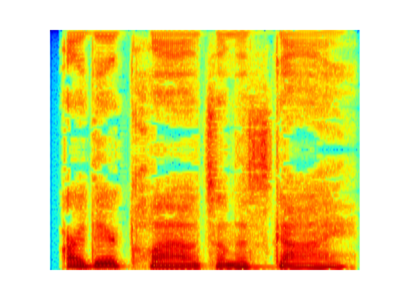
\includegraphics[width=0.2\textwidth]{3_noise0.png}};
\node[inner sep=0.5pt, label=below:are there clouds on sky] (3n30)  [right=4mm of 2n30] {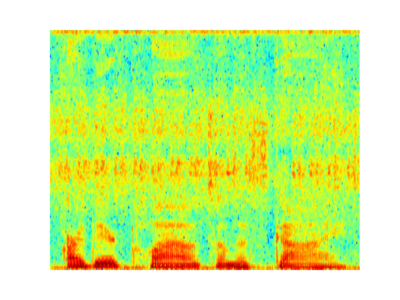
\includegraphics[width=0.2\textwidth]{3_noise30.png}};
\node[inner sep=0.5pt, label=below:are there files on the sky] (3n50)  [right=4mm of 2n50] {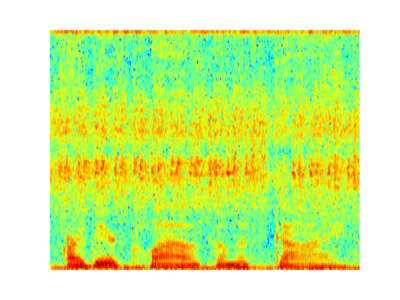
\includegraphics[width=0.2\textwidth]{3_noise50.png}};
\node[inner sep=0.5pt, label=below:are there clouds on the sky] (3r)  [right=4mm of 2r] {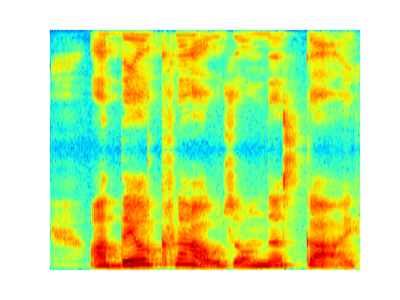
\includegraphics[width=0.2\textwidth]{3_recorded.png}};

\node (-center) [empty, label=\textbf{0\% Noise}]  (n0label)  [left=2mm of 1n0]     {};
\node (-center) [empty, label=\textbf{30\% Noise}] (n30label) [left=2mm of 1n30]    {};
\node (-center) [empty, label=\textbf{50\% Noise}] (n50label) [left=2mm of 1n50]    {};
\node (-center) [empty, label=\textbf{Human}]      (hmlabel)  [left=2mm of 1r]      {};

\draw (-2.3,-1) -- (-2.3,-17);
\draw (2.3,-1) -- (2.3,-17);
\end{tikzpicture}
\caption{Spectrograms for 3 example questions with corresponding transcribed text below. 3 synthetically generated and 1 human-recorded audio clips for each question.}
\label{fig:specs}
\end{figure}

We also make an additional, supplementary study of the practicality of speech-based VQA with real data. 1000 questions from the \textit{val} set were randomly selected and recorded with human speakers. Two speakers (one male and one female) participated the recording task. In total, 1/3 of the data is from a male speaker, the rest is from a female speaker. Both speakers are graduate students who are not native anglophones. The data was recorded in an office environment, and there are various background noises in the audio clips as they naturally occurred.

\section{Experiments}
\label{sec:experiment}
For SpeechMod, the only preprocessing step is to scale each waveform to a range of [-256, 256] as done by \cite{soundnet}. There was no need to center each example around 0, as they are already centered.

For TextMod, the standard preprocessing steps from \cite{VQA} were followed. This tokenizes each question, and replaces each token with a number that corresponds to the word’s index. These number indices are used as input, since the question will be fed to the model as a sequence of one hot encodings. Because questions have different lengths, an encoding mask of 0 is used as padding for sequences that are too short. The 0 encoding essentially causes the model to skip that position. 0 is also used for unseen tokens, which is especially useful when dealing with out of vocabulary words during evaluation.

We use Kaldi \cite{kaldi} for ASR, due to its open-source codebase and popularity with the speech research community. There are many pre-trained models available, but the one used in this work is a chain model, released by API.ai.\footnote{https://github.com/api-ai/api-ai-english-asr-model} Conveniently, it is trained on assistant.ai logs (essentially short commands) making it suitable to predict short utterances such as the questions in the \textit{VQA 1.0}.

Word error rate (WER) is used to measure the accuracy of speech to text transcriptions. WER is defined as follows: 
\begin{displaymath}
  \mathit{WER} = (S+D+I)/N
\end{displaymath}
Where \textit{S} is the number of substitutions, \textit{D} is the number of deletions, and \textit{I} is the number of insertions. \textit{N} is the total number of words in the sentence being translated. Each transcribed question is compared with the original; the results are shown in \Cref{table:wer}. WER is not expected to be a perfect measure of transcription accuracy, since some words are more essential to the meaning of a sentence than other words. E.g. missing the word \emph{dog} in the sentence \emph{what is the dog eating} is more detrimental than missing the word \emph{the}, but we nevertheless employ it to convey a general notion of how many words are understood by the ASR. Naturally the more noise there is, the higher the word error rate becomes. Due to transcription errors, there are resulting questions that contain words not seen in the original datasets. These words, as mentioned above, are indexed as 0 and are masked when fed into the system.


\begin{table}[t]
\centering
\caption{Word Error Rate from Kaldi speech recognition}
\label{table:wer}
\begin{tabular}{c|c}
Noise (\%)   & WER (\%) \\ \hline
0  & 8.46  \\
10 & 12.37 \\
20 & 17.77 \\
30 & 25.41 \\
40 & 35.15 \\
50 & 47.90
\end{tabular}
\end{table}


Keras was used to run all experiments, with the adam optimizer for both architectures. No parameter tuning was done; the default adam parameters are as follows: learning rate=0.001, beta1=0.9, beta2=0.999, epsilon=1e-08, learning  rate decay=0.0. Training TextMod for 10 epochs on \textit{train} + \textit{val} takes roughly an hour on a Nvidia Titan X, and our best model was taken at 30 epochs. Training SpeechMod for 10 epochs takes roughly 7 hours. The reported model is taken at 30 epochs. The code is made available to the public.\footnote{Will be provided after review}

Results are reported on \textit{test-dev} and are trained on \textit{train} + \textit{val}, shown in \Cref{table:vqa test-dev}. The standard format of reporting \textit{VQA 1.0} are followed: All is the overall accuracy, Y/N is for questions with yes or no as answers, Number is for questions that are answered by counting, and Other covers the rest.

TextMod is trained on the original questions, and the best performing model on \textit{OQ} (original question) is selected. ASR is used on the 0-50\% variants to convert the audio question to text, then the selected model from \textit{OQ} is used to evaluate based on the transcribed text. Likewise, SpeechMod is first trained on audio data with 0\% noise, and the strongest model on 0\% \textit{test-dev} is selected. The selected model is used to evaluate on the 10-50\% variants.

\textit{Blind} denotes no visual information, meaning it removes the visual components while rest of the model stays the same. TextMod \textit{Blind} is trained and evaluated on the original questions. SpeechMod \textit{Blind} is trained and evaluated on the 0\% noise audio. Conversely, \textit{I Only} denotes using visual information only, with no linguistic components of the model.

A graphical version of the table is shown in \Cref{fig:noiseplots}. The constant values of SpeechMod \textit{Blind} and TextMod \textit{Blind} are included to show the noise level at which they perform better than their SpeechMod and TextMod counterparts. Visual examples of the two models can be seen in \Cref{fig:visual:examples}.


\begin{table}[t]
\centering
\caption{Accuracy on test-dev with different levels of noise added. (Higher the better)}
\label{table:vqa test-dev}
\begin{tabular}{ll|cccc}
          &                     & All    & Y/N    & Number & Other \\ \hline
          & I Only \cite{VQA}   & 28.13  & 64.01  & 00.42  & 3.77  \\ \hline
TextMod   & Blind               & 48.76  & 78.20  & 35.68  & 26.59 \\
          & OQ                  & 56.71  & 79.17  & 34.63  & 42.53 \\
          & 0\%                 & 53.83  & 75.97  & 33.56  & 39.52 \\
          & 10\%                & 52.11  & 74.41  & 32.90  & 37.43 \\
          & 20\%                & 49.69  & 71.53  & 32.22  & 34.99 \\
          & 30\%                & 46.30  & 67.86  & 30.96  & 31.38 \\
          & 40\%                & 42.60  & 64.92  & 27.41  & 26.98 \\
          & 50\%                & 38.74  & 63.05  & 23.4   & 21.47 \\ \hline
SpeechMod & Blind               & 42.05  & 79.17  & 34.63  & 19.84 \\ 
          & 0\%                 & 46.99  & 67.87  & 30.84  & 32.82 \\
          & 10\%                & 45.81  & 67.29  & 30.13  & 31.03 \\
          & 20\%                & 43.58  & 66.08  & 29.06  & 27.66 \\
          & 30\%                & 40.35  & 64.71  & 26.84  & 22.62 \\
          & 40\%                & 36.10  & 61.98  & 24.97  & 16.54 \\
          & 50\%                & 32.25  & 59.64  & 20.54  & 11.48 
\end{tabular}
\end{table}


Finally, we ran a small, supplementary test on non-synthetic, human generated questions to see if the models would perform differently on real-world audio inputs. The results are shown in \Cref{table:recorded}. The 1000 samples were randomly selected from the val set, since ground truth from the \textit{test-dev} and \textit{test} are withheld and cannot be evaluated partially on the server. The models were trained on \textit{train}, and the highest performing on \textit{val} is selected to use as evaluation on the 1000 samples. The word error rate when transcribing this subset is 38.26\%.


\section{Discussion}
\label{sec:discussion}
\subsection{Results}

To logically reason about the results, we make the assumption that spoken language as a modality contains more information than written language. When going from a mode of high information to one of lesser, i.e. high dimensional spaces to lower dimensional spaces, information must be loss, or be preserved at best. Conversely, when transforming from a mode to another richer in information, information can be preserved easily, but cannot be gained. Thus, running TextMod with \textit{OQ} can be understood as the upper bound of all the models. Any transformations from the original, clean text to speech can only result in information loss. When the original textual inputs are replaced with transcribed inputs from a recognition system, the performance worsens as adding more noise obfuscates the system's linguistic understanding.

More interesting is to compare the performance of TextMod and SpeechMod while treating audio as their starting point, instead of the original text. They both falter at similar rates with added noise, though TextMod beats SpeechMod by a seemingly consistent margin of 6\%-7\%. One might imagine SpeechMod to perform better due to its direct optimization and end-to-end training solely for the task, yet this hypothesis does not hold.

In the process of reducing the high dimensional audio inputs to the low dimensional class output label, i.e. the answer, the best performing system must be the one that extracts patterns most effectively (provided there are such patterns in the data). TextMod relies heavily on the intermediate ASR system, which typically is magnitudes more complicated than the entire architecture of SpeechMod, and the number of parameters one needs to learn for a speech recognition is also much greater. Many ASRs include feature extractors at the encoding phase, wide and deep central architectures, acoustic models, language models in the decoding phase, and have been trained on thousands of times more data than contained in \textit{VQA 1.0}. The ASR serves to filter out noise in high dimensions and extract meaningful patterns in the form of text. From the results we must conclude that indirect as it may be, using ASR to obtain text first is more useful and informative than the end-to-end approach.


\pgfplotsset{width=8cm,compat=1.9}
\begin{figure}[t]
\centering
\begin{tikzpicture}
\begin{axis}[
    title={},
    xlabel={Noise (\%)},
    ylabel={Accuracy (\%)},
    xmin=0, xmax=50,
    ymin=30, ymax=60,
    xtick={0,10,20,30,40,50},
    ytick={30,40,50,60},
    legend pos=north east,
    legend style={font=\fontsize{6}{6}\selectfont}
]
 
\addplot[
    color=blue,
    mark=square,
    ]
    coordinates {
    (0,46.99)(10,45.81)(20,43.58)(30,40.35)(40,36.10)(50,32.25)
    };
\addplot[
    color=magenta,
    mark=halfcircle,
    mark options={solid},
    dashed
    ]
    coordinates {
    (0,53.83)(10,52.11)(20,49.69)(30,46.3)(40,42.6)(50,38.74)
    };
\addplot[mark=none, color=blue] coordinates{(0,42.05) (50,42.05)};
\addplot[mark=none, color=magenta, dashed] coordinates{(0,48.76) (50,48.76)};
\legend{SpeechMod, TextMod, SpeechMod Blind 0\% Noise, TextMod Blind \textit{OQ}}
 
\end{axis}
\end{tikzpicture}
\caption{SpeechMod and TextMod performance with varying amounts of added noise. \textit{Blind} counterparts are not tested on different noise levels.}
\label{fig:noiseplots}
\end{figure}


\begin{figure*}[ht]
$\begin{tabular}{cccc}
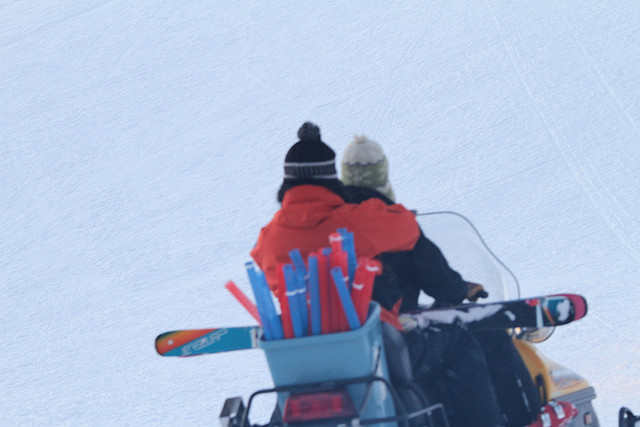
\includegraphics[width=0.24\linewidth, height=30mm]{images/howmany.jpg}
& \hspace{-3mm}
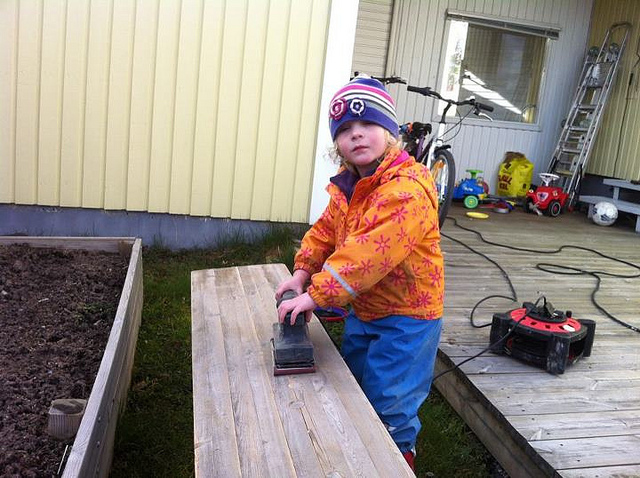
\includegraphics[width=0.24\linewidth, height=30mm]{images/lean.jpg}
& \hspace{-3mm}
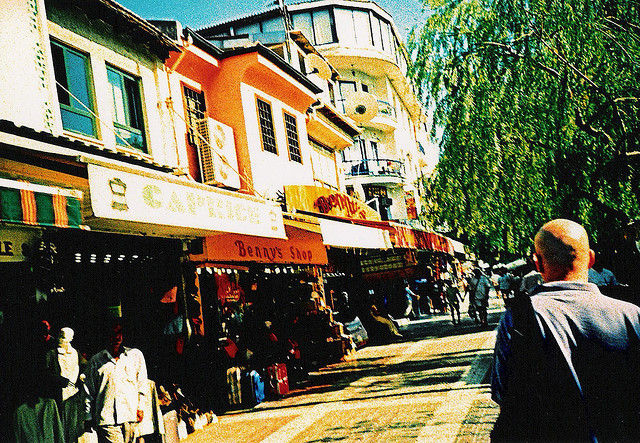
\includegraphics[width=0.24\linewidth, height=30mm]{images/spanish.jpg}
& \hspace{-3mm}
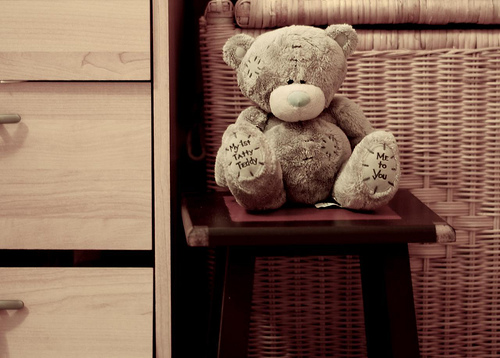
\includegraphics[width=0.24\linewidth, height=30mm]{images/teddy.jpg}

\\
\vspace{-3mm}
\begin{tcolorbox}[width=0.24\linewidth, left=1pt,right=1pt,top=0pt,bottom=0pt]
how many people are in this photo? 
\end{tcolorbox}
%}
& \hspace{-3mm}
\begin{tcolorbox}[width=0.24\linewidth, left=1pt,right=1pt,top=0pt,bottom=0pt]
what is leaning against the house?
\end{tcolorbox}
%}
& \hspace{-3mm}
%\multirow{ 2}{*}{
\begin{tcolorbox}[width=0.24\linewidth, left=1pt,right=1pt,top=0pt,bottom=0pt]
is this a spanish town?
\end{tcolorbox} 
& \hspace{-3mm}
\begin{tcolorbox}[width=0.24\linewidth, left=1pt,right=1pt,top=0pt,bottom=0pt]
what is the teddy bear sitting on? 
\end{tcolorbox}  \\

\vspace{-5mm}
\\
\begin{tcolorbox}[width=0.24\linewidth, left=1pt,right=1pt,top=0pt,bottom=0pt]
 TextMod \ityping: {\color{blue} 2} \\
 SpeechMod \ispeaking: {\color{blue} 2} 
\end{tcolorbox}
%}
& \hspace{-3mm}
\begin{tcolorbox}[width=0.24\linewidth, left=1pt,right=1pt,top=0pt,bottom=0pt]
TextMod \ityping: {\color{red} yes} \\
SpeechMod \ispeaking: {\color{red} chair} 
\end{tcolorbox}
%}
& \hspace{-3mm}
%\multirow{ 2}{*}{
\begin{tcolorbox}[width=0.24\linewidth, left=1pt,right=1pt,top=0pt,bottom=0pt]
TextMod \ityping: {\color{red} no} \\
SpeechMod \ispeaking: {\color{blue} yes} 
\end{tcolorbox} 
& \hspace{-3mm}
\begin{tcolorbox}[width=0.24\linewidth, left=1pt,right=1pt,top=0pt,bottom=0pt]
TextMod \ityping: {\color{blue} chair} \\
SpeechMod \ispeaking: {\color{red} yes} 
\end{tcolorbox}  \\
%\text{\textbf{(a) Relevance}} &  
%\text{\textbf{(b) Coverage}} & 
%\text{\textbf{(c) Perspective}} &
%\text{\textbf{(d) Knowledge }} 
\end{tabular}$
\vspace{-4mm}
\caption{Example of speech-based VQA answers. Correct answers in blue and incorrect in red.}  
\label{fig:visual:examples} 
\end{figure*}


It is important to note the reasoning above and the conclusion does not discourage nor invalidate the end-to-end method. In contrast to the characteristics of the pipelined approach, SpeechMod does not explicitly include mechanisms that learn semantics in language, and the only data it learns from is the given dataset. Bearing in mind its simple architecture and limited amount of data, we find the performance gap of 7\% between SpeechMod and TextMod to be well within acceptable limits and to merit further study into the end-to-end methods.

Next, we direct the reader's attention to comparing TextMod and SpeechMod against their respective \textit{Blind} models. It is documented in \cite{VQA} and \cite{VQA2} the type of bias in \textit{VQA 1.0}. Namely, if the question is understood, there is a good chance of answering correctly without looking at the image. For example, Y/N questions have the answer \emph{yes} more commonly than \emph{no}, so the system should guess \emph{yes} if a question is identified to be a Y/N type. Therefore, \textit{Blind} tells us how many questions are understood by these two modes of linguistic inputs. When comparing the linguistic only models with their complementary TextMod and SpeechMod, one can be certain that performances falling below the linguistic signifies that the model no longer understands the questions. Furthermore, perceiving the image and a noisy question becomes less informative than perceiving a clean question by itself.

\begin{table}[t]
\centering
\caption{Performance on 1000 human recorded questions.}
\label{table:recorded}
\begin{tabular}{l|cccc}
                        & All   & Y/N   & Number & Other \\ \hline
SpeechMod (Recorded)    & 21.46 & 57.26 & 0.77   & 0.91  \\
SpeechMod (Synthetic)   & 42.69 & 66.58 & 32.31  & 27.58 \\ \hline
TextMod (Recorded)      & 41.66 & 66.33 & 35.69  & 25.37 \\
TextMod (Original Text) & 53.09 & 77.73 & 41.54  & 38.26
\end{tabular}
\end{table}

Lastly, we analyze the results from the 1000 recorded samples. Although small in sample size, the human-recorded dataset provides a few insights. For SpeechMod, the performance on synthetic data serves as the upper bound and for TextMod, the performance on the original text also serves the upper bound. Although it is clear that both models have difficulties handling non-synthetic audio inputs, SpeechMod performs especially poorly. The synthetic audio sounds monotonous, disinterested, with little silence in between words while the human recorded audio has inflections, emphasis, accents, and pauses. An inspection of the spectrograms (\Cref{fig:specs}) confirms this, as the synthetic waveforms contain less variance. Because SpeechMod uses the waveforms as input directly and it has no training data similar to the human recorded samples, during prediction time it is unable to find salient patterns in the audio clips. By comparison, the pipelined approach has an ASR that is already trained with data containing lots of variance, so it is able to normalize the waveform into a compact, salient textual representation before feeding it into TextMod. From the perspective of TextMod, its linguistic input is only slightly different than the original text it was trained on.

There are weaknesses and strengths associated with both approaches. Data is easier to find for the pipelined approach. There are plenty of speech data paired with transcripts, with different speech patterns and levels of noise but it is difficult to find speech data specific to an end application such as question answering. We saw that SpeechMod is sensitive to slight changes in the audio input, and one may expect that it finds patterns that cannot be extracted from textual input. Should the task be sentiment analysis or disambiguation, the end-to-end approach may very well be the better choice. However, \textit{VQA 1.0} is an objective dataset; the questions are objective and direct. There is no more information to be gained in the modality of speech that isn't contained in text, and thus the pipelined approach has the advantage. TextMod is also faster to train and run by many factors, as textual inputs exist in lower dimensional spaces than auditory inputs, and the model contains fewer parameters to learn.


\subsection{Future Work}

One straightforward approach to improving the end-to-end model is by data augmentation. It is widely accepted that effectiveness of neural architectures is data driven, so training with noisy data and different speakers will make the model more robust to inputs during run time. Just as many possibilities exist in improving the architecture. One can add feature extractors, attention mechanisms, or any amalgamation of the techniques in the deep learning mainstream.

\section{Conclusion}
\label{sec:conclusion}

We propose speech-based visual question answering and introduce two approaches that tackle this problem, one of which can be trained end-to-end on audio inputs. Despite its simple architecture, the end-to-end method works well when the test data has audio signatures comparable to its training data. Both methods suffer performance decreases at similar rates when noise is introduced. A pipelined method using an ASR tolerates varied inputs much better because it normalizes the input variance into text before running the VQA module. We release the speech dataset and invite the multimedia research community to explore the intersection of speech and vision.

\bibliographystyle{aaai}
\bibliography{sigproc} 

\end{document}
